\subsection{Xử lý ngôn ngữ tự nhiên}
\subsubsection{Định nghĩa}
Xử lý ngôn ngữ tự nhiên (Natural language processing - NLP) là một lĩnh vực phụ liên ngành của khoa học máy tính và tìm kiếm thông tin. Mục tiêu chính của nó là cung cấp cho máy tính khả năng hỗ trợ và thao tác với ngôn ngữ của con người. NLP liên quan đến việc xử lý các tập dữ liệu ngôn ngữ tự nhiên, chẳng hạn như kho văn bản hoặc kho dữ liệu giọng nói, bằng cách sử dụng các phương pháp học máy dựa trên quy tắc hoặc xác suất (tức là thống kê và gần đây nhất là dựa trên mạng nơ-ron). Mục tiêu là giúp máy tính có khả năng "hiểu" nội dung của các tài liệu, bao gồm cả sắc thái theo ngữ cảnh của ngôn ngữ trong đó. Vì mục đích này, xử lý ngôn ngữ tự nhiên thường vay mượn các ý tưởng từ ngôn học lý thuyết. Sau đó, công nghệ có thể trích xuất chính xác thông tin và hiểu biết có trong tài liệu, cũng như phân loại và tổ chức các tài liệu đó.

Những thách thức trong xử lý ngôn ngữ tự nhiên thường liên quan đến nhận dạng giọng nói, hiểu ngôn ngữ tự nhiên và tạo ngôn ngữ tự nhiên.

NLP có nguồn gốc từ những năm 1940 khi Alan Turing đã xuất bản một bài báo có tựa đề "Computing Machinery and Intelligence" đề xuất thứ hiện nay được gọi là Bài kiểm tra Turing làm tiêu chuẩn cho trí thông minh, mặc dù vào thời điểm đó nó không được coi là một vấn đề riêng biệt so với trí tuệ nhân tạo. Bài kiểm tra được đề xuất bao gồm một nhiệm vụ liên quan đến việc giải nghĩa và tạo ra ngôn ngữ tự nhiên một cách tự động. Sau đó quá trình phát triển của NLP gồm có 3 giai đoạn chính:

\begin{itemize}
    \item Symbolic NLP (1950 – đầu 1990): Tiền đề của NLP được trình bày bởi thí nghiệm Chinese Room của John Searle: Cung cấp cho máy tính một bộ quy tắc (ví dụ: sách hội thoại tiếng Trung, với các câu hỏi và câu trả lời tương ứng), máy tính mô phỏng khả năng hiểu ngôn ngữ tự nhiên (hoặc các tác vụ NLP khác) bằng cách áp dụng các quy tắc đó vào dữ liệu nó gặp phải.
    \item Statistical NLP (1990s–2010s): Cho đến những năm 1980, hầu hết các hệ thống xử lý ngôn ngữ tự nhiên đều dựa trên các bộ quy tắc phức tạp được viết bằng tay. Tuy nhiên, bắt đầu từ cuối những năm 1980, đã có một cuộc cách mạng trong lĩnh vực xử lý ngôn ngữ tự nhiên với việc đưa ra các thuật toán học máy cho xử lý ngôn ngữ. Điều này là do sự gia tăng ổn định về sức mạnh tính toán (định luật Moore) và sự giảm dần vai trò thống trị của các lý thuyết ngôn ngữ học theo Chomsky, những lý thuyết này không khuyến khích ngôn ngữ học dựa trên kho dữ liệu (corpus linguistics) - nền tảng của phương pháp học máy trong xử lý ngôn ngữ ngày nay.
    \item Neural NLP (hiện tại): Vào năm 2003, mô hình n-gram là thuật toán thống kê tốt nhất để xử lý ngôn ngữ tự nhiên. Tuy nhiên,Yoshua Bengio cùng các cộng sự đã vượt qua mô hình này bằng cách sử dụng mạng Perceptron đa lớp (có một lớp ẩn và khả năng xử lý ngữ cảnh của nhiều từ, được huấn luyện trên 14 triệu từ). Đến năm 2010, Tomáš Mikolov (khi đó là nghiên cứu sinh tiến sĩ tại Đại học Công nghệ Brno) cùng các cộng sự đã áp dụng mạng nơ-ron hồi quy đơn giản với một lớp ẩn vào xử lý ngôn ngữ. Sau đó, ông tiếp tục phát triển Word2vec. Và như thế, trong những năm tiếp theo của thập kỉ, việc học biểu diễn và các phương pháp học máy theo phong cách mạng nơ-ron sâu (có nhiều lớp ẩn) đã trở nên phổ biến trong lĩnh vực xử lý ngôn ngữ tự nhiên. 
\end{itemize}

\subsubsection{Các bước xử lý trong xử lý ngôn ngữ tự nhiên}

Phân tích hình thái: Đây là bước đầu tiên trong xử lý văn bản, nhằm nhận biết, phân tích và miêu tả cấu trúc của từng đơn vị ngôn ngữ, chẳng hạn như từ gốc, biên từ, phụ tố, từ loại, v.v. Các bài toán điển hình trong phần này là tách từ (word segmentation) và gán nhãn từ loại (part-of-speech tagging) trong xử lý tiếng Việt. 

Phân tích cú pháp: Phân tích cú pháp là quá trình phân tích một chuỗi các biểu tượng ngôn ngữ theo cú pháp của ngôn ngữ. Đầu vào là một câu văn và đầu ra là một cây phân tích thể hiện cấu trúc cú pháp của câu đó. Các phương pháp thường dùng trong phân tích cú pháp là văn phạm phi ngữ cảnh (context-free grammar - CFG), văn phạm danh mục kết nối (combinatory categorial grammar - CCG), và văn phạm phụ thuộc (dependency grammar - DG). 

Phân tích ngữ nghĩa: Phân tích ngữ nghĩa nhằm tìm ra ý nghĩa của các đơn vị ngôn ngữ và xác định mối quan hệ ngữ nghĩa giữa chúng, từ cấp độ từ vựng đến cấp độ cú pháp. Điều này liên quan đến việc hiểu được các từ và câu trong bối cảnh ngữ nghĩa của chúng.
 
Phân tích diễn ngôn: Phân tích diễn ngôn xem xét mối quan hệ giữa ngôn ngữ và ngữ cảnh sử dụng, thực hiện ở mức đoạn văn hoặc toàn bộ văn bản thay vì chỉ ở mức câu. Điều này giúp hiểu rõ hơn ý nghĩa và tầm quan trọng của một đoạn văn trong ngữ cảnh tổng thể của văn bản. 

\subsubsection{Một vài ứng dụng của xử lý ngôn ngữ tự nhiên}

Xử lý ngôn ngữ tự nhiên được ứng dụng rộng rãi trong nhiều khía cạnh của cuộc sống và công việc. Trong suốt hơn nửa thế kỷ, NLP đã phát triển đáng kể và đem lại nhiều ứng dụng đột phá. 

\begin{figure}[htb]
    \centering
    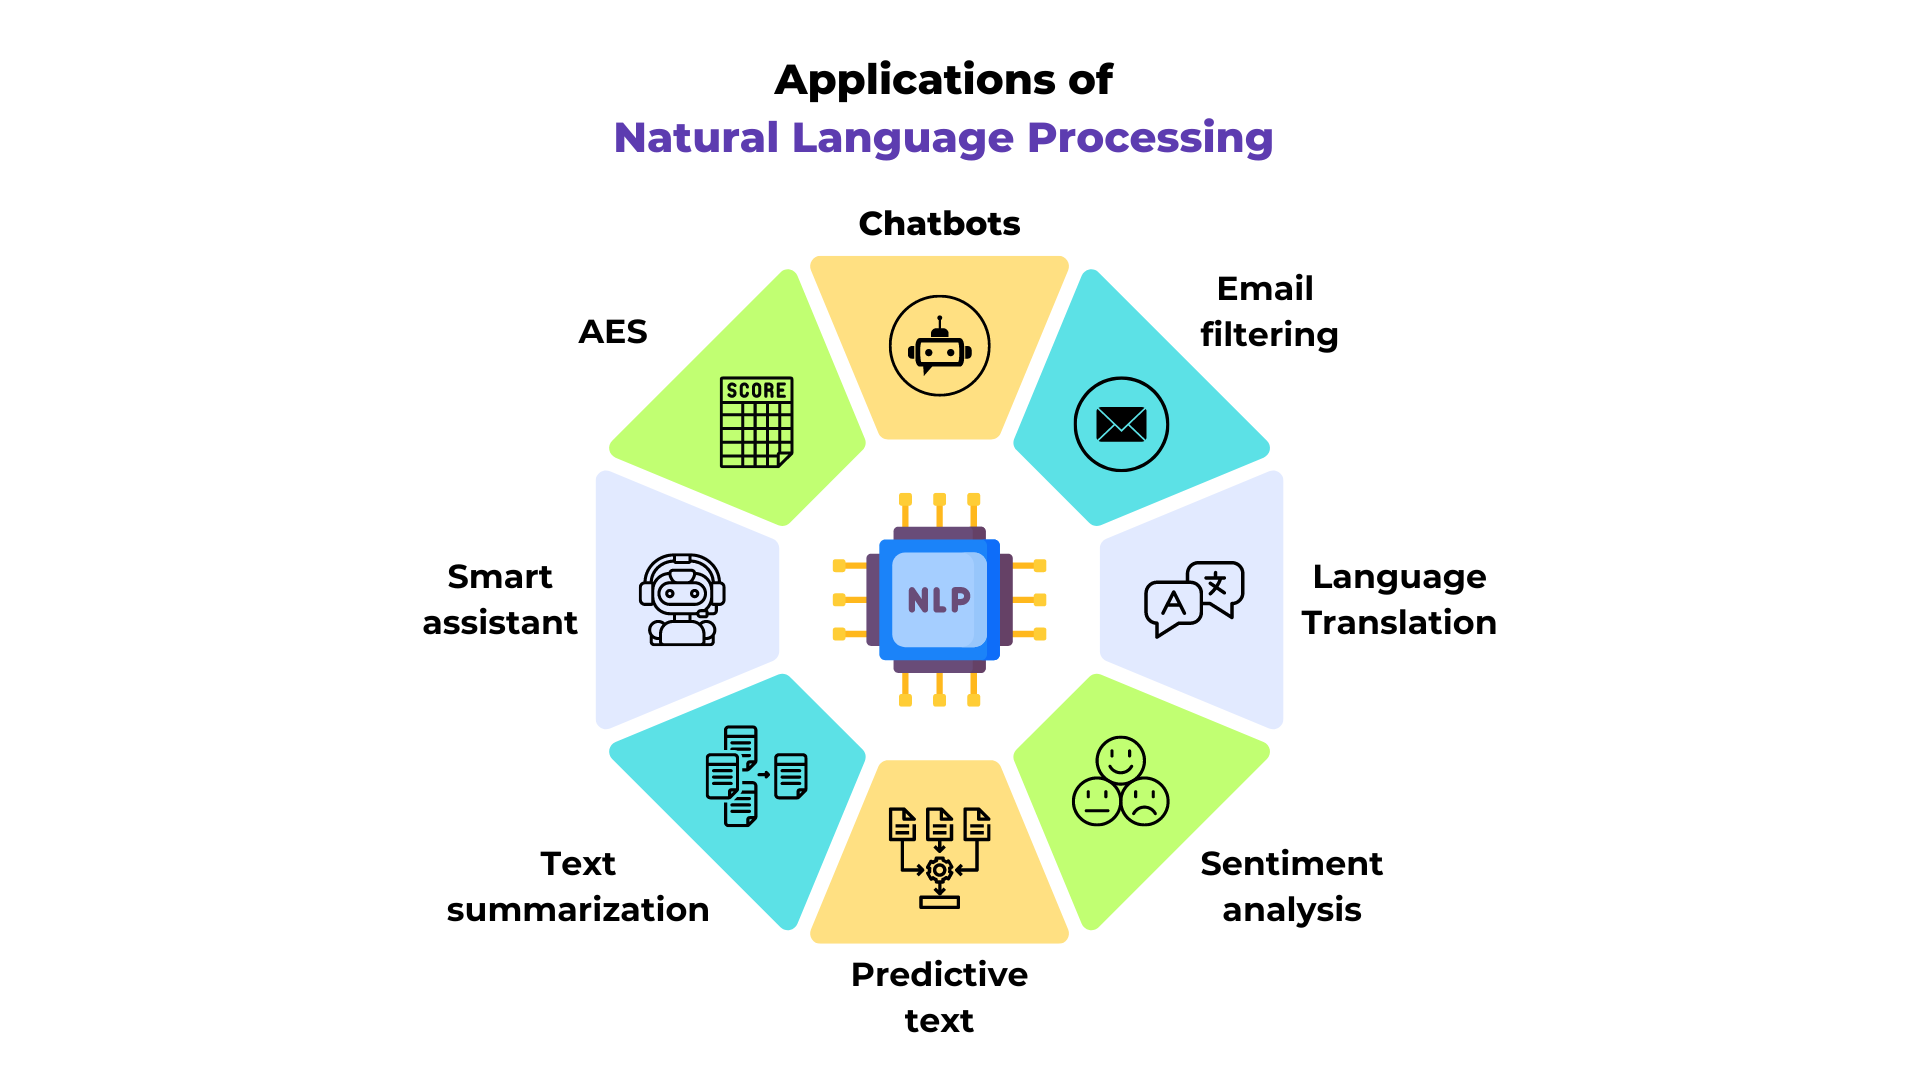
\includegraphics[width=\textwidth]{image/applications-of-nlp.png}
    \caption{Minh họa một số ứng dụng của xử lý ngôn ngữ tự nhiên}
    \label{fig:applications-of-nlp}
    % \source{https://www.analyticsvidhya.com/blog/2021/06/what-is-nlp-and-its-applications/}'
\end{figure}

\begin{itemize}
    \item Nhận dạng giọng nói (Automatic Speech Recognition - ASR, hoặc Speech To Text - STT) là một trong những ứng dụng tiêu biểu của xử lý ngôn ngữ tự nhiên. Với sự tiến bộ của các thuật toán và công nghệ, việc chuyển đổi từ tiếng nói sang văn bản đã trở nên chính xác hơn. Hệ thống nhận dạng giọng nói ngày càng phổ biến trong các ứng dụng hỗ trợ khách hàng, điều khiển thiết bị qua giọng nói và ghi chú cuộc họp.
    \item Tổng hợp giọng nói (Speech synthesis hoặc Text to Speech – TTS) là một ứng dụng ngược lại, cho phép máy tính đọc văn bản một cách tự nhiên và sinh động. Công nghệ tổng hợp giọng nói đang ngày càng tiến xa, giúp giọng nói của các chatbot và trợ lý ảo trở nên sống động và giống thực tế hơn, tạo sự tương tác tự nhiên và gần gũi hơn với con người.
    \item Trả lời câu hỏi (Question Answering - QA) là một bài toán phức tạp trong xử lý ngôn ngữ tự nhiên, yêu cầu máy tính hiểu và trả lời câu hỏi dưới dạng ngôn ngữ tự nhiên. Một hệ thống QA hiệu quả cần kết hợp các phương pháp như trích xuất thông tin, phân tích ngữ pháp và xử lý ngữ nghĩa. Đối với những câu hỏi đơn giản, hệ thống trả lời câu hỏi có thể đưa ra câu trả lời chính xác. Tuy nhiên, với những câu hỏi phức tạp hơn hoặc yêu cầu hiểu sâu hơn, các thách thức vẫn còn tồn tại và đòi hỏi sự phát triển thêm của xử lý ngôn ngữ tự nhiên. 
    \item Tóm tắt văn bản tự động (Automatic Text Summarization) là một ứng dụng quan trọng trong việc thu gọn và tóm tắt thông tin quan trọng từ văn bản gốc. Có hai phương pháp chính trong tóm tắt, là trích xuất và tóm lược ý. Trong trích xuất, hệ thống sẽ chọn các câu hoặc đoạn văn từ văn bản gốc, giữ lại những thông tin quan trọng nhất. Trong tóm lược ý, hệ thống sẽ tạo ra những câu tóm tắt mới dựa trên ngữ cảnh của văn bản. 
    \item Chatbot là một trong những ứng dụng phổ biến nhất của xử lý ngôn ngữ tự nhiên. Nhờ vào sự tiến bộ của các mô hình học máy và xử lý ngôn ngữ tự nhiên, chatbot ngày càng trở nên thông minh và có khả năng giao tiếp một cách tự nhiên. Chatbot được sử dụng trong nhiều lĩnh vực như hỗ trợ khách hàng, dự đoán thời tiết, đặt lịch hẹn và nhiều ứng dụng thú vị khác. 
    \item Dịch máy (Machine Translation - MT) là một trong những ứng dụng cổ điển nhất và đồng thời cũng là một trong những thách thức lớn trong xử lý ngôn ngữ tự nhiên. Với sự ra đời của mô hình dịch máy sử dụng mạng nơ-ron (neural machine translation), chất lượng dịch ngày càng được cải thiện và có thể đáp ứng nhu cầu của người dùng trong nhiều tình huống giao tiếp quốc tế. 
    \item Tạo hình ảnh từ văn bản (Text-to-image generation): Mô hình này có khả năng nhận dạng mô tả bằng ngôn ngữ tự nhiên và tạo ra hình ảnh tương ứng với mô tả đó. Sự phát triển của các ứng dụng này bắt đầu vào giữa những năm 2010, cùng với sự bùng nổ của Trí tuệ Nhân tạo (AI) nhờ những tiến bộ trong lĩnh vực mạng nơ-ron sâu. Đến năm 2022, chất lượng đầu ra của các mô hình tiên tiến như DALL-E 2 của OpenAI, Imagen của Google Brain, Stable Diffusion của Stability AI và Midjourney đã được đánh giá là gần tương đương với ảnh chụp thực tế và tranh vẽ của con người.
    \item Phân tích cảm xúc: Phân tích cảm xúc được sử dụng để xác định và phân loại ý định cảm xúc ẩn chứa trong văn bản. Kỹ thuật này bao gồm việc phân tích văn bản để xác định xem cảm xúc được thể hiện là tích cực, tiêu cực hay trung lập. Các mô hình phân loại cảm xúc thường sử dụng các đầu vào như chuỗi n-gram của từ, đặc trưng do con người tạo hoặc sử dụng các mô hình học sâu được thiết kế để nhận dạng cả các phụ thuộc dài hạn và ngắn hạn trong chuỗi văn bản. Ứng dụng của phân tích cảm xúc rất đa dạng, mở rộng sang các nhiệm vụ như phân loại đánh giá của khách hàng trên các nền tảng trực tuyến khác nhau.
\end{itemize}



\subsection{Kỹ thuật nhúng từ \textit{(Word embedding)}}
\subsubsection{Vấn đề đặt ra}
Máy móc vốn không thể hiểu được ngôn ngữ của con người, do vậy mà để máy móc xử lí ngôn ngữ thì chúng ta cần phải xử lí dữ liệu trước. Thông thường chúng ta có một số cách biểu diễn từ như sau: \cite{webpage13}
\begin{itemize}
    \item Biểu diễn từ dưới dạng một con số.
    \item Sử dụng one-hot encoding.
    \item Sử dụng word embedding.
\end{itemize}

Thông thường, trong học máy, các từ sẽ được biểu diễn dưới dạng one-hot encoding, dữ liệu của các từ sẽ được chuyển về dạng các vector với số chiều tương ứng với tổng số từ. Tuy nhiên cách thể hiện one-hot encoding có một số vấn đề: \cite{webpage12}
\begin{itemize}
    \item Chi phí lớn: Do số chiều của vector tương ứng với tổng số từ trong dữ liệu, độ phức tạp của vector có thể rất lớn, kéo theo đó là chi phí tính toán và lưu trữ.
    \item Không chứa thông tin: Do chỉ được biểu diễn dưới dạng vector mang hầu như chỉ số $0$, các từ sau khi đưa về dạng one-hot encode hầu như không mang thông tin giá trị hay sự liên kết giữa các từ với nhau.
    \item Thiếu đi sự khái quát: Trong ngôn ngữ thì có rất nhiều từ có nghĩa giống nhau, và khi biểu diễn bằng one-hot encoding sẽ không thể thể hiện sự giống nhau này.
\end{itemize}

Đối với cách biểu diễn với những con số, đây tuy là một cách đơn giản và tiết kiệm chi phí, tuy nhiên lại có thể dẫn tới sai lệch về sự liên quan giữa các từ. Ví dụ từ ``mèo'' được thể hiện với số $1$ và ``chó'' với số $2$, chúng ta sẽ nhận được kết quả: ``mèo'' + ``mèo'' = ``chó''. Đây là một ví dụ nhỏ về sự sai lệch khi biểu diễn dưới dạng số. \cite{webpage13}

Ở word embedding, kỹ thuật này gán mỗi từ với một vector, và các từ có quan hệ với nhau cũng được tính toán để các vector cũng có thể thể hiện được quan hệ tương đồng của các từ.

\subsubsection{Giới thiệu}
Word Embedding là một không gian vector dùng để biểu diễn dữ liệu có khả năng miêu tả được mối liên hệ, sự tương đồng về mặt ngữ nghĩa, văn cảnh(\textit{context}) của dữ liệu. Không gian này bao gồm nhiều chiều và các từ trong không gian đó mà có cùng văn cảnh hoặc ngữ nghĩa sẽ có vị trí gần nhau. Ví dụ như ta có hai câu : ``Hôm nay ăn táo'' và ``Hôm nay ăn xoài''. Khi ta thực hiện Word Embedding, ``táo'' và ``xoài'' sẽ có vị trí gần nhau trong không gian chúng ta biễu diễn do chúng có vị trị giống nhau trong một câu. \cite{webpage12}

\subsubsection{Một số phương pháp}
Có 2 phương pháp chủ yếu được sử dụng trong word embedding là Count based method và Predictive method. Các phương pháp này đều dựa trên một giả thuyết đó là những từ nào xuất hiện cùng nhau trong một ngữ cảnh sẽ có vị trí gần nhau trong không gian vector. \cite{webpage12}
\begin{enumerate}
    \item Count-based method: Phương pháp này tính toán mức liên quan về mặt ngữ nghĩa giữa các từ bằng cách thống kê số lần đồng xuất hiện của một từ so với các từ khác. Ví dụ chúng ta có 2 câu: ``Data is next oil'' và ``Data is future'', dựa trên 2 câu này chúng ta có thể tạo nên một ma trận tần suất đồng thời ở bảng \ref{table:frequency-matrix}. Từ bảng có thể thấy hai từ ``oil'' và ``future'' có vị trí khá gần nhau trên không gian vector.
    \item Predictive method: Khác so với Count-based method, Predictive method tính toán sự tương đồng ngữ nghĩa giữa các từ để dự đoán từ tiếp theo bằng cách đưa qua một mạng neural network có một hoặc vài layer dựa trên input là các từ xung quanh (\textit{context word}). Một context word có thể là một hoặc nhiều từ khác nhau. Chúng ta sẽ đi sâu hơn khi tìm hiểu phần tiếp theo, Word2vec.
\end{enumerate}

\begin{figure}[htb]
    \centering
    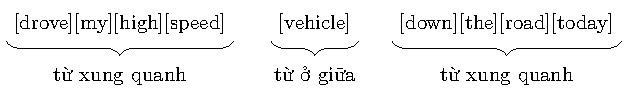
\includegraphics[width=0.7\textwidth]{tikz_image/predictive_method.pdf}
    \caption{Từ được dự đoán và các từ xung quanh}
    \label{figure:predictive-method}
\end{figure}

\subsection{Mô hình Word2vec}
Trong nhiều ứng dụng NLP (\textit{natural language processing}), các từ thường chỉ được biểu diễn bởi one-hot encoding và không giữ được quan hệ giữa các từ. Lí do để lựa chọn one-hot encoding là sự đơn giản và hiệu quả của chúng. \cite{Aggarwal2022-xj} Tuy nhiên với sự cải thiện của lĩnh vực học máy, các thuật toán phức tạp được huấn luyện trên các tập dữ liệu lớn đã hoạt động hiểu quả hơn các mô hình đơn giản. Tiêu biểu là thuật toán Word2vec có thể nắm bắt được cả sự tương đồng giữa ngữ pháp và ngữ nghĩa của các từ ngữ. Và một ví dụ được biết đến rộng rãi của Word2vec là:
\[
    \overline{King}-\overline{Man}=\overline{Queen}-\overline{Woman}
\]

\begin{figure}[htb]
    \centering
    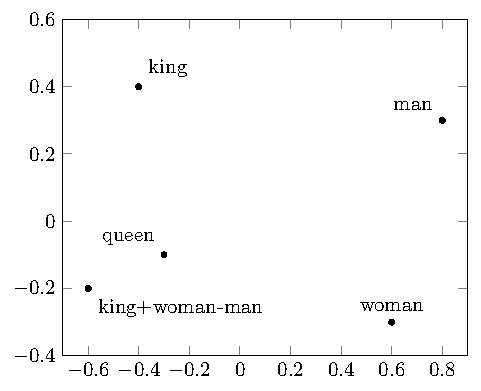
\includegraphics[width=0.6\textwidth]{tikz_image/word2vec_example.pdf}
    \caption{Ví dụ về Word2vec}
    \label{figure:word2vec-example}
\end{figure}

\subsubsection{Hoạt động của Word2vec}
Word2vec có 2 biến thể: dự đoán từ dựa trên các từ xung quanh - Continous Bag Of Words (CBOW) và dự đoán các từ xung quanh skip-gram.

Trong mô hình CBOW, các tập huấn luyện là các cặp từ có liên quan đến nhau, khi một tập các từ được nhập vào và một từ sẽ được đoán ra. Các từ nhập vào bao gồm $2\cdot t$ từ tương ứng với $t$ từ đứng trước và $t$ từ phía sau từ đó. Từ đó, tổng số các từ nhập vào sẽ là $m = 2\cdot t$ từ. Để đơn giản, các từ đầu vào sẽ được đánh là $w_1, w_2,\dots w_m$  và từ được dự đoán là $w$. Từ $w$ có thể có $d$ giá trị khả thi với $d$ là tổng số từ trong toàn tập huấn luyện. Mục đích của neural embedding là tính xác suất $P(w|w_1,w_2,\dots w_d)$ với $d$ là số từ trên toàn tập huấn luyện và tối ưu hóa xác suất đó trên toàn tập dữ liệu.
\begin{figure}[htbp]
    \centering
    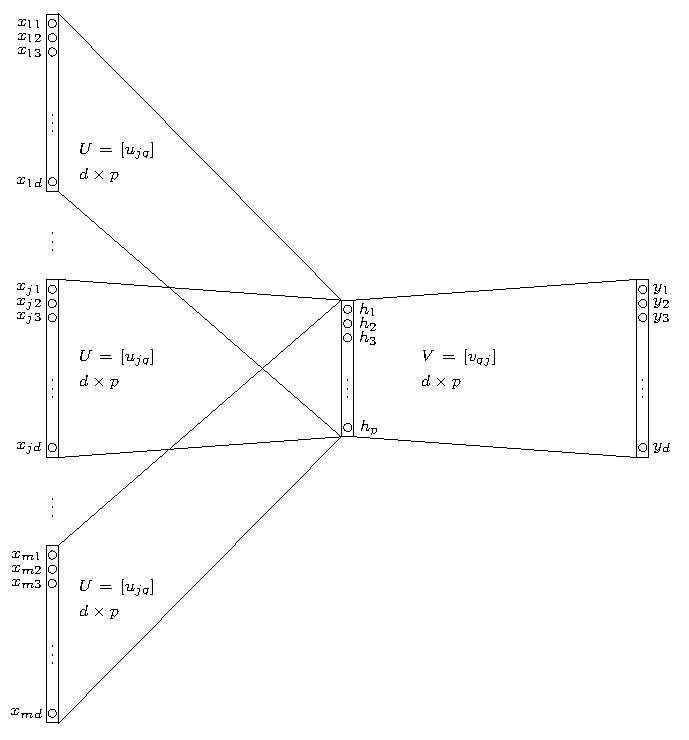
\includegraphics[width=0.7\textwidth]{tikz_image/word2vec_cbow.pdf}
    \caption{Cách hoạt động của CBOW \cite{Aggarwal2022-xj}}
    \label{figure:word2vec-cbow}
\end{figure}

Kiến trúc mỗi tầng được mô tả như sau: \cite{Aggarwal2022-xj}
\begin{itemize}
    \item Lớp đầu vào (\textit{input layer}): Kiến trúc tổng quát được mô tả ở hình trên. Đầu vào có $m$ từ tương ứng với $m$ vector, mỗi vector có $d$ chiều tương ứng với $d$ từ trong tập huấn luyện, từ đó ta có tổng cộng $m\cdot d$ nút đầu vào. Mỗi vector đầu vào sẽ được biểu diễn dưới dạng mã hoá one-hot. Chỉ một trong số $d$ của vector có giá trị là $1$ và còn lại sẽ có giá trị là $0$.
    \item Lớp ẩn (\textit{hidden layer}): Lớp ẩn chứa $p$ thành phần với $p$ là số chiều của Word2vec. Đầu ra của lớp ẩn là  $h_1,h_2,\dots h_p$. Lớp đầu vào được kết nối tới lớp ẩn bởi ma trận trọng số $U$ kích thước $d\cdot p$ như đã minh họa ở hình %.
\end{itemize}

Mỗi vector $\mathbf u_j = [u_{j1}, u_{j2},\dots,u_{jp}]$ là một nhúng $p$ chiều cho từ thứ $j$ trong toàn bộ từ đầu vào. vector $\mathbf h = [h_1,h_2,\dots,h_p]$ cung cấp một nhúng cho đầu vào. Từ đó đầu ra của lớp ẩn là trung bình các nhúng các từ nhập vào và được thể hiện dưới công thức:
\begin{align}
    \mathbf h=\dfrac{1}{m}\sum_{i=1}^m\sum_{j=1}^d\mathbf u_j\cdot x_{ij}
\end{align}
Và kết quả $\mathbf h$ được dùng để dự đoán kết quả đầu ra là một trong $d$ từ trong tập từ huấn luyện. Trọng số của đầu ra là ma trận $V = [v{jq}]$ kích thước $d\times p$. Với hàng thứ $j$ trong ma trận được biểu thị dưới dạng $\mathbf v_j$. Nhưng do ma trận kết nối tầng ẩn với đầu ra (\textit{hidden-to-output}) là một ma trận dạng $p\times d$, nó sẽ được biểu diễn dưới dạng $V^\intercal$. kết quả của việc nhân $\mathbf h$ với ma trận $V^\intercal$ tạo ra một vector $[\mathbf h\cdot\mathbf v_1,\dots,\mathbf h\cdot \mathbf v_d]$. Kết quả cho ra là kết quả của hàm softmax để tính xác suất mỗi nút của $y_1,\dots,y_d$.
\begin{align}
    \hat y_j=P(y_j=1|w_1\dots w_m)=\dfrac{\exp(\mathbf h\mathbf v_j)}{\sum_{k=1}^d\exp(\mathbf h\mathbf v_k)}
\end{align}

Trong mô hình Skip-gram, từ đầu vào được dùng để dự đoán m từ trước và sau. Từ đó chúng ta có $1$ input và $m$ output.
\begin{figure}[htbp]
    \centering
    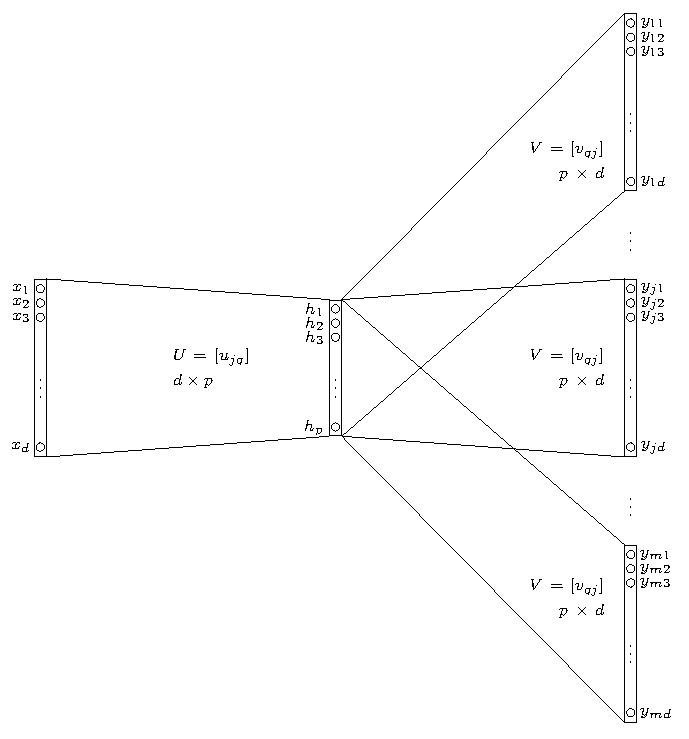
\includegraphics[width=0.7\textwidth]{tikz_image/word2vec_skipgram.pdf}
    \caption{Cách hoạt động của skip-gram}
    \label{figure:word2vec-skip-gram}
\end{figure}

Mô hình Skip-gram sử dụng một từ đầu vào $w$ và đầu ra là $m$ từ xung quanh được đánh là $w_1,\dots,w_m$. Do đó mục tiêu của skip-gram là tìm ra $P(w_1,\dots,w_m|w)$ khác với $P(w|w_1,\dots,w_m)$ của mô hình CBOW. Giống như trong CBOW, skip-gram cũng sử dụng mã hoá one-hot cho đầu vào và đầu ra của mô hình. Sau khi mã hoá chúng ta sẽ có vector $d$ chiều $[x1,\dots,x_d]$ tương ứng với $d$ giá trị khả thi cho một giá trị đầu vào. Tương tự như vậy, có $m$ vector đầu ra. Lớp ẩn có $p$ thành phần và có kết quả $[h_1\dots h_p]$. Lớp đầu vào kết nối với lớp ẩn bởi một ma trận $U$ kích thước $d\times p$.

Lớp ẩn được tính bởi ma trận $U = [u_{jq}]$ với kích thước $d\times p$:
\begin{align}
    \mathbf h=\sum_{j=1}^d \mathbf u_j\cdot x_j
\end{align}

Lớp ẩn kết nối tới lớp đầu ra bởi một ma trận $V=[v_{jq}]$ kích thước $d\times p$. Nhưng do ma trận kết nối từ lớp ẩn tới lớp đầu ra là dạng $p\times d$ nên ở đây sử dụng ma trận $V^\intercal$.
\begin{align}
    \hat y_{ij}=P(y_{ij}=1|w)=\dfrac{\exp(\mathbf h\cdot\mathbf v_j)}{\sum_{k=1}^d\exp(\mathbf h\cdot\mathbf v_k)}\quad\forall i\in\{1\dots m\}
\end{align}

\subsection{Mô hình GloVe}
\subsubsection{Giới thiệu}
Ở GloVe, chúng ta có thể trích xuất được mối quan hệ giữa các từ bằng cách sử dụng ma trận tần suất đồng thời (\textit{co-occurrence matrix}). Với một câu có $U$ từ thì ma trận tần suất đồng thời $X$ sẽ có dạng $U\cdot X$. Trong ma trận này hàng thứ $i$ và cột thứ $j$ sẽ biểu diễn giá trị $X_{ij}$ thể hiện sự cùng xuất hiện của hai từ tại vị trí cột $i$ và hàng $j$.

Ví dụ chúng ta có 2 câu: ``Data is next oil'' và ``Data is future''. Dựa trên 2 câu này chúng ta có thể tạo nên một ma trận tần suất đồng thời.
\begin{table}[htb]
    \centering
    \caption{Ma trận tần suất đồng thời \cite{webpage9}}
    \label{table:frequency-matrix}
    \begin{tabular}{ l c c c c c }
        \toprule
               & Data & is & next & oil & future \\\midrule
        Data   & 0    & 2  & 0    & 0   & 0      \\
        is     & 2    & 0  & 1    & 0   & 1      \\
        next   & 0    & 1  & 0    & 0   & 0      \\
        oil    & 0    & 1  & 0    & 1   & 0      \\
        future & 0    & 0  & 1    & 0   & 0      \\
        \bottomrule
    \end{tabular}
\end{table}

Xác suất $P(j|i) = X_{ij}/X_i$ là xác suất mà từ tại hàng $j$ xuất hiện đồng thời với cột $i$. Như có thể thấy, xác suất để từ ``Data'' xuất hiện khi có từ ``is'' là $P(\text{Data|is}) = 2/4$. Với một ví dụ khác
\begin{table}[htb]
    \centering
    \caption{Xác suất các từ cùng xuất hiện \cite{webpage9}}
    \begin{tabular}{ l c c c c }
        \toprule
                                            & \multicolumn{4}{c}{k}                                                                   \\\cmidrule{2-5}
                                            & solid                 & gas                 & water               & fashion             \\\midrule
        $P(\text{k|ice})$                   & $1.9\times 10^{-4}$   & $6.6\times 10^{-5}$ & $3.0\times 10^{-3}$ & $1.7\times 10^{-5}$ \\
        $P(\text{k|steam})$                 & $2.2\times 10^{-5}$   & $7.8\times 10^{-4}$ & $2.2\times 10^{-3}$ & $1.8\times 10^{-5}$ \\
        $P(\text{k|ice})/P(\text{k|steam})$ & $8.9$                 & $8.5\times 10^{-2}$ & $1.36$              & $0.96$              \\
        \bottomrule
    \end{tabular}
\end{table}

Với bảng trên, chúng ta có thể thấy tỉ lệ chất rắn (\textit{solid}) xuất hiện với băng đá (\textit{ice}) cao hơn hẳn tỉ lệ chất khí (\textit{gas}) với băng đá (\textit{ice}). Như vậy, khi các từ có liên quan đến nhau, tỉ lệ đồng xuất hiện sẽ cao, ngược lại khi không liên quan, tỉ lệ đồng xuất hiện của các từ sẽ thấp. Nhưng khi một từ cùng liên quan tới nhiều từ, ví dụ nước (\textit{water}) đều liên quan tới băng đá (\textit{ice}) và hơi nước (\textit{steam}), do vậy trong những trường hợp này tỉ lệ nhận được sẽ khá cao. Để xử lí vấn đề này, chúng ta sử dụng $P_{ik}/P_{jk}$.

Tuy nhiên khi ứng dụng ma trận này trực tiếp, chúng ta sẽ gặp vấn đề nếu dữ liệu có hàng triệu chiều. Do đó, GloVe sử dụng ma trận tần suất đồng thời cùng với Word2vec để xử lí vấn đề trên.
\begin{align}
    F(w_i,w_j,\tilde w_k)=\dfrac{P_{ik}}{P_{jk}}
\end{align}

Ở công thức trên có $3$ vector từ $i,j,k$ với $k$ là vector của các từ được nhập vào. Và hàm $F$ tính xác suất các từ cùng xuất hiện với nhau.

Ở đây chúng ta có một vấn đề, đó là ở phương trình trên, phía bên trái chứa các vector trong khi số bên phải là một con số tỉ lệ. Do đó chúng ta cần chuyển đổi các vector thành các đại lượng vô hướng.
\begin{align}
    \label{eq:glove-prob}
    F((w_i-w_j)^\intercal,\tilde w_k)=\dfrac{P_{ik}}{P_{jk}}
\end{align}

Để chuyển đổi vector thành các đại lượng vô hướng, chúng ta thường sử dụng điểm tích của hai vector. Tuy nhiên ở đây chúng ta có $3$ vector, do đó chúng ta lấy hiệu của hai vector $i$ và $j$. Từ phương trình \ref{eq:glove-prob}, với $F(w_i^\intercal\tilde w_k)=P_{ik}=X_{ik}/X_i$, ta có
\begin{align}
    F((w_i-w_j)^\intercal,\tilde w_k)=\dfrac{F(w_i^\intercal\tilde w_k)}{F(w_j^\intercal\tilde w_k)}
\end{align}

\subsection{Mô hình Fasttext}
Các phương pháp như Word2vec và GloVe tạo ra các vector khác nhau đại diện cho từ trong kho các từ huấn luyện. Tuy nhiên các phương pháp này lại không thể tìm được sự liên kết giữa các từ dựa trên sự giống nhau giữa các từ. Có nhiều ngôn ngữ mà các từ ngữ đồng nghĩa được biến đổi từ một từ ban đầu, từ đó chúng ta có thể cải thiện được mô hình vector của những ngôn ngữ đó bằng thông tin ở mức kí tự.

Fasttext có thể được coi là một sự mở rộng của Word2vec, tuy nhiên khác với Word2vec hoạt động ở mức độ các từ riêng biệt, Fasttext hoạt động ở mức n-gram kí tự đối với mỗi từ. Ví dụ chúng ta có từ ``apple'' và $n = 3$ thì n-gram của từ này là: <ap, app, ppl, ple, le> và <apple>. Và vector đại diện cho từ ``apple'' có thể được tính bằng tổng các vector n-gram của chính nó.

Giống với Word2vec, Fasttext cũng hoạt động dựa trên 2 phương pháp:
\begin{itemize}
    \item Continous Bag Of Words (CBOW): Cách thức hoạt động tương tự như Word2vec, nhưng với mỗi từ được tính bằng n-gram. Ví dụ chúng ta có câu: ``I want to learn fast text'', các từ ``I'', ``want'', ``to'', ``fast'', ``text'' được cung cấp để mô hình dự đoán từ ``learn'' (hình \ref{figure:fasttext-cbow}).
    \item Skip-gram: Với ví dụ tương tự phía trên, chúng ta áp dụng skip-gram sẽ như hình \ref{figure:fasttext-skip-gram}.
\end{itemize}
\begin{figure}[htbp]
    \centering
    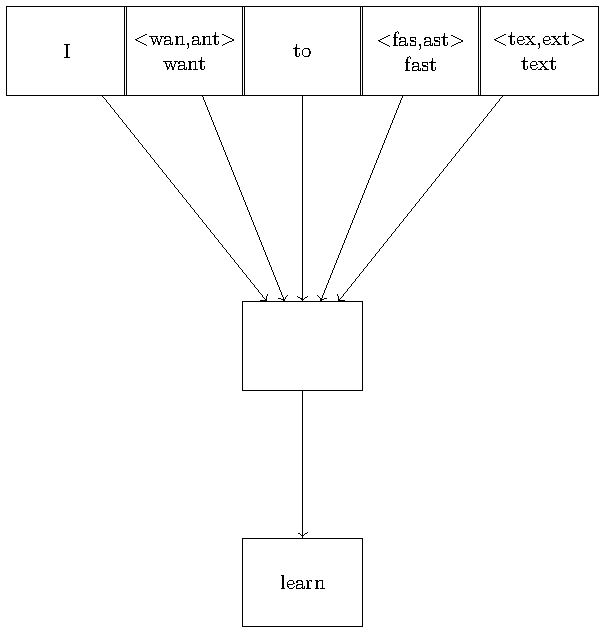
\includegraphics[width=0.7\textwidth]{tikz_image/fasttext_cbow.pdf}
    \caption{Mô hình fasttext đối với CBOW \cite{webpage14}}
    \label{figure:fasttext-cbow}
\end{figure}
\begin{figure}[htbp]
    \centering
    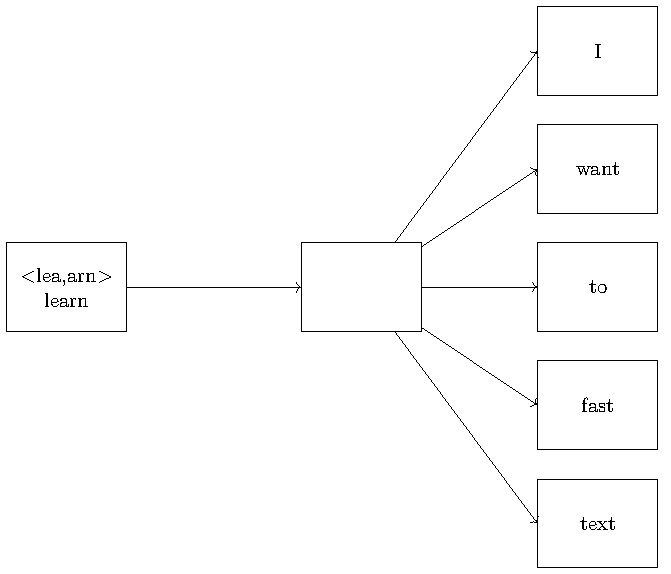
\includegraphics[width=0.7\textwidth]{tikz_image/fasttext_skipgram.pdf}
    \caption{Mô hình fasttext đối với skip-gram \cite{webpage14}}
    \label{figure:fasttext-skip-gram}
\end{figure}
